\section{Difficulties}

\subsection{Coupling}
Coupling is the cyclic dependency between units to be tested.

In large software projects, components are usually dependent on one another.
For example, the dependency graph of a web server might look like figure \ref{fig:depweb}.

\begin{figure}
	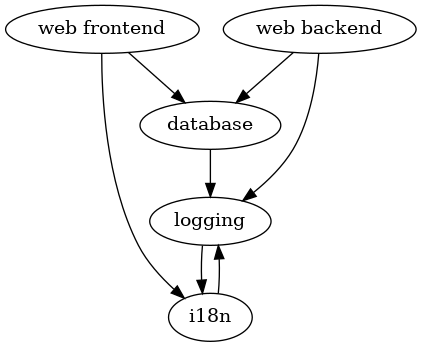
\includegraphics[width=3in]{example-deps.png}
	\caption{Dependency graph of a web server}
	\label{fig:depweb}
\end{figure}

A relation worth noting is between logging and i18n.
I18n requires a logger to log its loading process,
and logger requires i18n to display proper messages.
While this is complicated to write from the beginning,
it is even harder to unit test,
because it is not possible to only unit test logger without having a functional i18n component.

In other words, it is not possible to decide which component to unit test first,
because both modules are mutually dependent.

This condition is called modular coupling. Common practices to prevent it include:

\paragraph{Abstraction}: Create an interface for logger and simulate a simple dummy logger to unit test i18n.
Create an interface for i18n and simulate a constant dummy i18n system to unit test logger.
\paragraph{Dependency mocking}As explained in the previous section, dependency mocking can be used to prevent dependencies while testing,
but there are many problems about dependency mocking too.

Therefore, the best solution to coupling is to prevent cyclic dependencies from the beginning.
